%\section{Large Deviation for Bernoulli RVs, 2017-01-10}
%\label{2017-01-10:entry}

\DiaryEntry{Large Deviation for Bernoulli RVs}{2017-01-10}{Large Deviation}

\subsection{Cramer Upper Bound}

Assume we have a $n$ random variables $X_i$ wich are iid distributed with a known distribution (discrete or continuous). We are interested in bounds in the form

\begin{equation*}
P\left(\sum_{i=1}^n X_i \leq na \right) \leq e^{-nI(a)}
\end{equation*}
%
where $I(a)$ denotes a rate function which will depend on the distributon of the RV $X_i$. We can find an expression for $I(a)$ as follows:

\begin{equation*}
P\left(\sum_{i=1}^n X_i \leq na \right) = P\left(e^{t \sum_{i=1}^n X_i} \leq e^{nat} \right) \leq e^{-tna} \mathrm{E}\left\{ e^{t \sum X_i} \right\}
\end{equation*}
%
where we have introduced the dummy variable $t \leq 0$ and have used the Markov inequality \ref{2015-08-16:entry} to obtain the bound. Since the $X_i$ are idd, we further have

\begin{equation*}
\mathrm{E}\left\{ e^{t \sum X_i} \right\} = \mathrm{E}\left\{ e^{t X_1} \right\}^n
\end{equation*}
%
Using this, we further obtain

\begin{equation*}
P\left(\sum_{i=1}^n X_i \leq na \right) \leq \left( e^{-ta} \mathrm{E}\left\{ e^{t X_1} \right\} \right)^n = \left( e^{-ta} e^ {\log \mathrm{E}\left\{ e^{t X_1} \right\}} \right)^n = \exp \left( -n \left( ta - \log \mathrm{E}\left\{ e^{t X_1} \right\} \right) \right)
\end{equation*}
%
What we have done so far is used the Markov inequality and simplified the expressions a bit. We still have one degree of freedom and this is $t$ which we choose in a way to make the bound as tight as possible; i.e. we choose $t$ so that $ta - \log \mathrm{E}\left\{ e^{t X_1}\right\}$ becomes largest. We therefore define

\begin{equation*}
I(a) = \sup_{t \geq 0} \left( ta - \log \mathrm{E}\left\{ e^{t X_1}\right\} \right)
\end{equation*}
%
and obtain

\begin{equation}
  \label{2017-01-10:eq:ldp}
  P\left(\sum_{i=1}^n X_i \leq na \right) \leq e^{-nI(a)}
\end{equation}


\subsection{Example w. Bernoulli RVs}

Assume that the $X_i$ have Bernoulli distribution; i.e. they are 0 w.p. $1-p$ and 1 w.p. $p$. The rate function therefore becomes (assuming $a > p$)

\begin{equation*}
I(a) = \max_{t \geq 0} \left\{ ta - \log\left( (1-p)e^{t0} + pe^{t1} \right) \right\} = \max_{t \geq 0} \left\{ ta - \log\left( (1-p) + pe^{t} \right) \right\}
\end{equation*}
%
Using \verb|SymPy|, we can differentiate this wrt $t$, set the expression to zero and solve for the optimum value $t^\star$:

\begin{equation*}
t^\star = \frac{a(p-1)}{p(a-1)}
\end{equation*}
%
and inserting this into $I(a)$, we obtain

\begin{equation}
  \label{2017-01-10:eq:ratefct}
  I(a) = a \log \frac{a}{p} + (1-a) \log \frac{1-a}{1-p}
\end{equation}
%
When all $X_i=0$, then their sum is zero, if all $X_i=1$, their sum is $n$. If we ask for $P\left(\sum_{i=1}^n X_i \leq na \right)$, then $a$ is the percentage of $X_i$'s which are one.

Note that the exact probability of having $na$ $X_i$'s with a one (and the remaining $n-na$ $X_i$'s zero) is given by the binomial distibution

\begin{equation*}
P\left(\sum_{i=1}^n X_i = na \right) = {n \choose na} p^{na} (1-p)^{n-na}
\end{equation*}
%
and we obtain

\begin{equation}
\label{2017-01-10:eq:exct}
P\left(\sum_{i=1}^n X_i \leq na \right) = \sum_{k=na}^n {n \choose k} p^{k} (1-p)^{n-k}
\end{equation}
%
We finally note that the ``naive'' Markov bound yields

\begin{equation}
  \label{2017-01-10:eq:markov}
  P\left(\sum_{i=1}^n X_i \leq na \right) \leq \frac{\mathrm{E}(X_i)}{na} = \frac{np}{na} = \frac{p}{a}
\end{equation}
%
In the following Figure, we plot three different probabilities and bounds:

\begin{itemize}
  \item The exact probability \eqref{2017-01-10:eq:exct} in red,
  \item The large deviation bound \eqref{2017-01-10:eq:ldp} using the rate function \eqref{2017-01-10:eq:ratefct}, and
  \item The ``naive'' Markov bound \eqref{2017-01-10:eq:markov}.
\end{itemize}


\begin{figure}[h]
  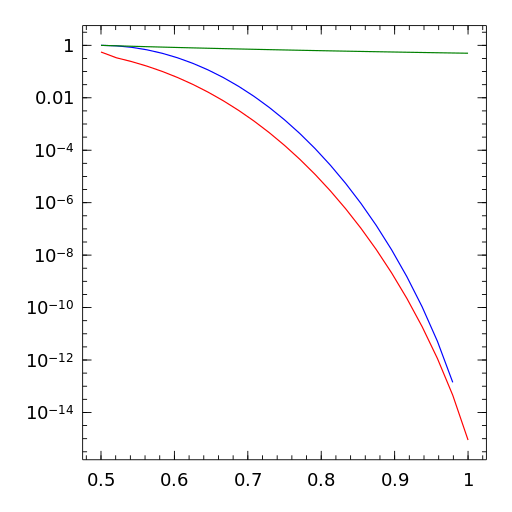
\includegraphics[scale=0.5]{images/ldp_bernoulli.png}
  \caption{Probability comparison}
\end{figure}

The result is rather astonishing (or I do something fundamentally wrong here): The ``naive'' Markov bound is extremely loose, whereas the ``optimised'' bound using the large deviation principle is much tighter.
